\documentclass{article}
\usepackage{graphicx} % Required for inserting images
\usepackage[T1]{fontenc}
\usepackage{amsmath}
\usepackage{hyperref}

\usepackage[section]{placeins}

% JAK BĘDZIEMY KOMPILOWAĆ FINAL TO TRZEBA OD ODKOMENTOWAĆ
\usepackage{fontspec}
\usepackage{polyglossia}
\setdefaultlanguage{polish}
\setmainlanguage{polish}
\PolyglossiaSetup{polish}{indentfirst=true}
% \setlength{\parindent}{0pt}


% kolorowe snippety -- ukradzione z https://www.overleaf.com/learn/latex/Code_listing
\usepackage{listings}
\usepackage{xcolor}

\definecolor{codegreen}{rgb}{0,0.6,0}
\definecolor{codegray}{rgb}{0.5,0.5,0.5}
\definecolor{codepurple}{rgb}{0.58,0,0.82}
\definecolor{backcolour}{rgb}{0.95,0.95,0.92}

\lstdefinestyle{mystyle}{
    backgroundcolor=\color{backcolour},   
    commentstyle=\color{codegreen},
    keywordstyle=\color{magenta},
    numberstyle=\tiny\color{codegray},
    stringstyle=\color{codepurple},
    basicstyle=\ttfamily\footnotesize,
    breakatwhitespace=false,         
    breaklines=true,                 
    captionpos=b,                    
    keepspaces=true,                 
    numbers=left,                    
    numbersep=5pt,                  
    showspaces=false,                
    showstringspaces=false,
    showtabs=false,                  
    tabsize=2
}


\lstset{
    style=mystyle,
    caption={Example Listing},
    % numbersep=5pt,
    % frame=single,
    % label=lst:example, % Default label (can be overridden)
}


\title{Port}
\author{Karol Tomczyk, Patryk Nogaś}
\date{Czerwiec 2026}

\begin{document}

\maketitle

\section{Wprowadzenie}

W naszym projekcie na podstawy podejmowania decyzji, zadecydowaliśmy się zamodelować problem optymalnego cumowania floty w porcie w którym są dwa doki, które są od siebie oddalone w taki sposób, że statki największe blokują przepływ wewnątrz do portu, taki przypadek również występuje wtedy, kiedy dwa średnie statki stoją na przeciwko siebie. Naszym celem jest maksymalizacja funkcji celu, która premiuje ilość statków, które zacumowały, ale również ma na uwadze to jak duży jest ten statek. Kluczowe oczywiście w modelu było też to, że nie może statek być w dwóch miejscach naraz, ani dwa statki nie mogą być w jednym miejscu. Akurat ostatnie zdanie to truizm, za który przepraszam.

\hfill

Podeszliśmy do problemu macierzowo, stworzyliśmy macierz decyzyjną. Można ją interpretować na wiele sposobów, jednym z nich jest myślenie że każdy statek ma swoją własną planszę/port \emph{$M[s_{1}]$}...[d][c], i wraz z wpływaniem kolejnych statków nakładamy, kolejne ograniczenia od $s_1$ do S, gwarantując poprawne rozwiązanie.

\hfill

Natomiast w metaheurystyce skorzystaliśmy z algorytmu genetyczny, algorytmu wprost wzorowanego na obserwacjach zjawisk w biologii. Przypomina on, jak zobowiązuje nazwa, ewolucję gatunków. Polega on na wylosowaniu dwóch rodziców (algorytmów), które potem posiadają dzieci z mutacjami jak z fallouta; Następnie mordujemy dzieci, które są porażkami życiowymi i zostawiamy te z najlepszymi rozwiązaniami (chromosomami).

\hfill

\raggedright{Kluczowe informacje}
\begin{itemize}
    \item Decydentem jest bosman portu
    \item Jest to system podejmowania decyzji.
    \item Wejściem jest lista staków, ilość miejsc do cumowania w każdym z docków i ilość docków która zawsze wynosi 2 (dla innych argumentów nie ma sensu).
    \item postacią wyjścia jest rozłożenie statków w porcie, przy lekkiej gimnastyce można policzyć też funkcję celu i np. procent statków przyjętych do portów, lecz nie jest to nasz priorytet. 
    \item Rozwiązanie przy korzystaniu z optymalizacji liniowej jest optymalne, rozwiązanie algorytmem ewolucyjnym nie musi być optymalne.
\end{itemize}



% \textcolor{purple}{SPRAWDZIĆ POWYŻSZE!}


\section{Forma matematyczna}


Dane:

- Typy statków:

\(typy \in {1,2,3}\)

- Liczba statków:
\(S = 12\)

- Liczba doków:

\(D = 2\)

- Liczba miejsc do cumowania w dokach:

\(C=10\)

- Lista statków:
\(L=[...]\)

Zmienne decyzyjne:

\begin{equation}
    M[N][D][C]
\end{equation}


Funkcja celu:
%  bez premiowania statków
% \begin{equation}
%     max \sum_{s=1}^{S} \sum_{d=1}^{D} \sum_{c=0}^{C} M[s][d][c]
% \end{equation}

\begin{equation}
    max \sum_{s=1}^{S} L[s] * (\sum_{d=1}^{D} \sum_{c=0}^{C} M[s][d][c])
\end{equation}

% MOŻLIWĄ koncepkcją jest też to aby zrobić dwie funkcje celu, jedna z premiowaniem statków druga bez premiowania. Wtedy przy maksymalizacji obu będziemy mieć po pierwsze najwięcej wartościowych statków, a w drugiej kolejności po prostu najwięcej statków w porcie.

Ograniczenia:

\begin{equation} \label{eq:uniq}
    \forall_{s\in S} ( \forall_{d\in D}\forall_{c \in C} M[n][d][s] \leq 1 )
\end{equation}

W \ref{eq:uniq} zapewniamy, że statek, będzie co najwyżej raz w porcie. 

\begin{equation} \label{eq:no-duplication}
    \forall_{d\in D}\forall_{c \in C} (\forall_{s \in S} M[n][d][s] \leq 1)
\end{equation}

W \ref{eq:no-duplication} zapewniamy, że nie ma dwóch statków w tym samym miejscu.

\begin{equation} \label{eq:3jka-blokuje}
    \begin{split}
        ((\forall_{s_1\in S}\forall_{d_1\in D}\forall_{c_1 \in C} M[s_1][d_1][c_1] \equiv 1) \land (L[s_1] \equiv 3 )) \implies  \\
    (\forall_{s_2>s_1} \forall_{d_2 \in D} \forall_{c_2 \leq c} M[s_2][d_2][c_2] \equiv 0)
    \end{split}
\end{equation}

W \ref{eq:3jka-blokuje} zapewniamy, że statek o wielkości 3 blokuje część wewnętrzną portu.

\begin{equation} \label{eq:2jka-blokuje}
    \begin{split}
        (((\forall_{s_1\in S}\forall_{d_1\in D}\forall_{c_1 \in C}  M[s_1][d_1][c_1] \equiv 1) \land (L[s_1] = 2 )) \land \\
        ( \exists_{s_2} M[s_2][ \neg d_1][c_1] = 1) \land ( L[s_2] \equiv 2 ))  ) \\
        \implies (\forall_{s_3>s_1} \forall_{d_2 \in D} \forall_{c_3 \leq c} M[s_3][d][c_3] \equiv 0)
    \end{split}
\end{equation}

W \ref{eq:2jka-blokuje} zapewniamy sobie, że dwa statki na przeciwko siebie również blokują wewnętrzną stronę portu.




\section{Implementacja w Pythonie\texttrademark}
Implementacja w pythonie nie jest zaskakująca.

Losujemy dane do zadania w ten sposób:
\begin{lstlisting}[language={Python}, label={lst:declare}, caption={Deklaracja i losowanie zmiennych}]
dlugosci_lodek = np.random.randint(0,4,20) # 4 bo randint jest exclusive
wartosc_za_lodke = {0:1, 1:6, 2:5, 3:4}
cena_za_lodke = {0:1, 1:60, 2:70, 3:90}
\end{lstlisting}

Następnie tworzymy model:
\begin{lstlisting}[language={Python}, label={lst:model}, caption={Macierz decyzyjna}]
N_lodek = len(dlugosci_lodek)


model = gp.Model("Optymalizacja_Macierzowa")

#Funkcja kary => Jezeli wystapi ograniczenie dwoch lodek nakładamy na funkcję celu karę 

M = model.addMVar(shape = (N_lodek,N_rzedow,N_slotow), vtype = GRB.BINARY, name= "Model portu do mapowania lodek")


f_cel = gp.quicksum(M[b,i,s] * (1 + wartosc_za_lodke[dlugosci_lodek[b]]) for b in range(N_lodek) for i in range(N_rzedow) for s in range(N_slotow)) 

model.setObjective(f_cel, GRB.MAXIMIZE)
\end{lstlisting}

Warto zauważyć, że powyżej posiadamy funkcję kary której nie ma w modelu matematycznym, została ona dodana, aby ujednolicić implementację obu rozwiązań, gdyż dla metaheurystyki jest ona konieczna.

\subsection{Ograniczenia}
W tym ograniczeniu \ref{lst:uniq}, zapewniamy unikalność \ref{eq:uniq}

\begin{lstlisting}[language={Python}, label={lst:uniq}, caption={Uniqueness}]
#kazda lodka w jednym slotcie

for b in range(N_lodek):
    model.addConstr(M[b,:,:].sum() <= 1)
\end{lstlisting}


Natomiast w tym ograniczeniu \ref{lst:no-duplication} zapewniamy, że \ref{eq:no-duplication} nie ma duplikacji.
\begin{lstlisting}[language={Python}, label={lst:no-duplication}, caption={No duplication}]
#kazdy slot przyjmuje tylko jedna lodke

for i in range(N_rzedow):
    for s in range(N_slotow):
        model.addConstr(M[:,i,s].sum() <= 1)
\end{lstlisting}


Dzięki korzystaniu z \verb|np.where|, udało nam się uprościć implementację modelu w kodzie.

Tutaj ~\ref{lst:3jka-blokuje} implementujemy \ref{eq:3jka-blokuje}.
\begin{lstlisting}[language={Python}, label={lst:3jka-blokuje}, caption={Statek wielkości 3 blokuje część portu}]
for boat_3 in np.where(dlugosci_lodek == 3)[0]:
    for i in range(N_rzedow):
        
                model.addConstr(
                    (M[boat_3,i,0] == 1) >> (M[:,i,1] == 0),
                    name = 'Zakaz stawania na przeciwko (dla lewej strony)'
                )

                model.addConstr(
                    (M[boat_3,i,1] == 1) >> (M[:,i,0] == 0),
                    name = 'Zakaz stawania na przeciwko (dla prawej strony)'
                )
\end{lstlisting}

Natomiast tutaj \ref{lst:2jka-blokuje} implementujemy \ref{eq:2jka-blokuje}

\begin{lstlisting}[language={Python}, label={lst:2jka-blokuje}, caption={Statek wielkości 2 blokuje część portu}]
boat_2 = np.where(dlugosci_lodek == 2)[0]

for i in range(N_rzedow - 1):
    for b1 in boat_2:
            for b2 in boat_2:
                if b1 != b2:
                    
                    z = model.addVar(vtype=GRB.BINARY, name='Wartosc blokady przez dwie lodki o dlugosci 2')

                    model.addConstr(z == gp.and_(M[b1,i,0], M[b2,i,1]))

                    model.addConstr((z==1) >> (M[:,i+1,:].sum() == 0))

\end{lstlisting}

I tak o to wyglądają kluczowe elementy implementacji w pythonie.

\subsection{Wyniki}

Seed dla wszystkich wyników w tej podsekcji wynosi 67.

\begin{lstlisting}[caption={Wyniki dla N\_rzedow = 10, N\_slotow = 2 i 20 łódek}]
[[1. 1.]
 [3. 0.]
 [2. 1.]
 [2. 1.]
 [0. 3.]
 [2. 1.]
 [1. 0.]
 [3. 0.]
 [0. 3.]
 [2. 1.]]
\end{lstlisting}

Funkcja celu wynosi 26 dla powyższego przypadku 

\begin{lstlisting}[caption={Wyniki dla N\_rzedow = 10, N\_slotow = 2 i 18 łódek}]
[[1. 2.]
 [3. 0.]
 [3. 0.]
 [1. 1.]
 [2. 1.]
 [1. 2.]
 [1. 1.]
 [0. 3.]
 [3. 0.]
 [0. 3.]]
\end{lstlisting}

Funkcja celu wynosi 28 dla powyższego przypadku.

\begin{lstlisting}[caption={Wyniki dla N\_rzedow = 10, N\_slotow = 2 i 16 łódek}]
[[1. 1.]
 [3. 0.]
 [0. 1.]
 [3. 0.]
 [1. 2.]
 [3. 0.]
 [0. 3.]
 [1. 1.]
 [0. 3.]
 [1. 2.]]
\end{lstlisting}

Funkcja celu wynosi 26 dla powyższego przypadku.

Widzimy, że wraz ze spadkiem ilości wszystkich łódek jest mniej łódek o długości 2 -- które są najbardziej optymalną kombinacją w naszych algorytmach, ale wcale nie widzimy straty w funkcji celu. Zwiększa się natomiast ilość łódek o długości 3.

\subsubsection{Ciekawe przypadki}

\begin{lstlisting}[caption={Wyniki dla N\_rzedow = 10, N\_slotow = 2 i 67 łódek}]
[[2. 1.]
 [1. 1.]
 [1. 2.]
 [1. 1.]
 [1. 1.]
 [1. 1.]
 [1. 2.]
 [1. 1.]
 [1. 1.]
 [1. 2.]]
\end{lstlisting}

Funkcja celu wynosi 24 dla powyższego przypadku. Nie wzrosła ona od przypadku z 22 i 20 łódkami, bo posiadamy funkcję kary. Nie warto zastanawiać się długo nad tym przypadkiem, bo raczej mało możliwe jest to że przypłynie ilość statków, która jest 3 krotnie większa niż jest miejsc w porcie.

\section{Algorytm Genetyczny}

Algorytm Genetyczny to metaheurystyka używana w problemach optymalizacji i podejmowania decyzji. Metoda ta wzorowana jest na biologicznej ewolucji, krzyżowaniu i mutowaniu genotypów. Genotyp składa się z chromosomów, który składa się z genów. W naszym modelu podejmowania decyzji za chromosom przyjęliśmy port, a należący do niego gen to łódka o znanej długości i pozycji w porcie (rząd i strona). Działanie algorytmu, z uwzględnieniem założeń projektowych, wygląda następująco:

\begin{enumerate}
    \item Losowana jest populacja. W tym przypadku będą to chromosomy, które odzwierciedlają przykładowe pozycje ułożenia statków (genów) w porcie.
    \item Populacja poddawana jest ocenie za pomocą pomocniczej funkcji fitness, której działanie odzwierciedla funkcję celu (blokady portu są karane, a dobre ustawienie premiowane). Najlepiej dopasowane chromosomy biorą udział w dalszym procesie ewolucyjnym
    \item Genotypy wybranych chromosów poddawane są:
    \begin{itemize}
    \item \textbf{Krzyżowaniu}: Dwa chromosomy dzielone są na 3 równe części. Wyciągany jest środek z jednego chromosomu i zamieniany jest ze środkiem drugiego. 
    \item \textbf{Mutacji}: Losowo wybrany gen zostaje zmieniony na inny. Przyporządkowywana jest mu inna pozycja w porcie. Ilość elementów poddawanych mutacji zależy od podanego prawdopodobieństwa zmian.
    \end{itemize}
    \item Rodzi się następne pokolenie. Populacja jest aktualizowana o chromosomy, których funkcja celu jest największa. Chromosomy o mniejszej wartości odpadają. Jeżeli nie znaleziono dobrego rozwiązania, algorytm powraca do kroku drugieg (ocena nowej populacji). W przeciwnym wypadku wybieramy najkepszego osobnika (chromosm) z populacji. Jego genotyp to nasze optymalne metaheurystyczne rozwiązanie. 
\end{enumerate}
    
\subsection{Wyniki}

Implementacja zaczyna się od stworzenia populacji początkowej. Odpowiedzialna jest za to funkcja generate chromosme (patrz Listing 12). W innym modelu generowana jest lista łodzi, które wiemy, że przybędą do portu.

\begin{lstlisting}[language={Python}, label={Generowanie listy łódek}, caption={Moduł odpowiadający za generowanie listy łódek}]

boat = [0,1,2,3]
wagi = [0.10, 0.35, 0.35, 0.20] 

wylosowany = random.choices(boat, weights=wagi, k=N_lodek)

print(wylosowany)
# [1, 1, 2, 2, 1, 1, 1, 3, 3, 3, 3, 3, 1, 1, 1, 3, 1, 3, 2, 2, 2]

stala_lista = [1, 1, 2, 2, 1, 1, 1, 3, 3, 3, 3, 3, 1, 1, 1, 3, 1, 3, 2, 2, 2]
    
\end{lstlisting}

Wartość stala-lista (patrz Listing 11) importowana jest do modułu metaheurystyki. Na jej podstawie funkcja generująca chromosomy będzie tworzyła populację początkową. W celu ochrony przed tworzeniem się powtarzających chromosomów, lista jest tasowana na samym wejściu do funkcji.

\begin{lstlisting}[language={Python}, label={Funkcja generowania chromosomów}, caption={Funkcja odpowiadająca za generowanie chromosomów}]

def generate_chromosome(idx_boat, N_lodek = 21, N_rzedow = N_rzedow, N_slotow=N_slotow):
    
    gene = []
    random.shuffle(idx_boat)

    zajete_sloty = set()
    zajete_przez_trojki = set()

    for b in idx_boat:
            
        wolne = []
        for i in range(N_rzedow):
            for j in range(N_slotow):
                if (i,j) in zajete_sloty:
                    continue
                if i in zajete_przez_trojki:
                    continue
                if b == 3:
                    if (i, 1 - j) in zajete_sloty:
                        continue
                wolne.append((i,j))
        if not wolne:
            continue
    
        rzad, strona = random.choice(wolne)
        gene.append(Gen(b, rzad, strona))
        zajete_sloty.add((rzad, strona))

        if b == 3:
            zajete_przez_trojki.add(rzad)

    return Chromosom(gene)

\end{lstlisting}


Przed wykonaniem kroków algorytmu trzeba było stworzyć funkcję odpowiedzialne za krzyżowanie, mutacje oraz obliczanie wartości fitness.


Zaczynamy od funkcji crossing, która przyjmuje dwa chromosomy rodziców, które wyprodukują dziecko. Dziecko to wynik krzyżowania oraz również nowy członek naszej populacji. Chromosomy dzielone są na 3 równe części. Zwracany jest nowy gen, który składa się z dwóch części chromosomu jeden oraz jednej cześci chromosomu 2.
\begin{lstlisting}[language={Python}, label={Funkcja krzyżowania}, caption={Funkcja odpowiadająca za krzyżowanie się chromosomów}]

def crossing(parent_a: Chromosom, parent_b: Chromosom):
    '''
    Crossing dzieli chromosomy na 3 czesci. Nastepnie zamienia srodkową czesc miedzy genami
    '''
    geny_a = parent_a.geny
    geny_b = parent_b.geny
    m = min(len(geny_a), len(geny_b))

    p1, p2 = sorted(random.sample(range(m), 2))

    segment = geny_a[p1:p2]
    zajete = {(g.rzad, g.strona) for g in segment}

    dopelnienie = [
        Gen(g.lodka, g.rzad, g.strona)
        for g in geny_b
        if (g.rzad, g.strona) not in zajete
    ]

    nowe_geny = dopelnienie[:p1] + segment + dopelnienie[p1:]

    return Chromosom(nowe_geny)

\end{lstlisting}

Funkcja mutacji w sposób losowy zamienia miejscami dwa geny w chromosomie. Prawdopodobieństwo tych zmian jest odgórnie ustalone przez wartośc prob, która bazowo nosi wartość 0.1. Zwracany jest chromosom z nowym układem genów.

\begin{lstlisting}[language={Python}, label={Funkcja mutacji}, caption={Funkcja odpowiedzialna za mutacje chromosomów}]

def mutation(chromosome: Chromosom, N_rzedow: int, prob=0.1):
    '''
    Wybieramy losowy gen z chromosomu i wybieramy dla niego nowe losowe miejsce
    '''
    geny = [Gen(g.lodka, g.rzad, g.strona) for g in chromosome.geny]

    for idx in range(len(geny)):
        if random.random() > prob:
            continue

        drugi_idx = random.randint(0, len(geny) - 1)
        if drugi_idx == idx:
            continue

        geny[idx].rzad, geny[drugi_idx].rzad = geny[drugi_idx].rzad, geny[idx].rzad
        geny[idx].strona, geny[drugi_idx].strona = geny[drugi_idx].strona,  geny[idx].strona

    return Chromosom(geny)

\end{lstlisting}

Funkcja fitness to pomocnicza funkcja, która działa podobnie jak funkcja celu. Oblicza ona wynik krzyżowania i mutacji dla przyjętych kryteriów. Według naszego modelu, funkcja karać będzie wszystkie chromosomy, w których występuje blokada reszty genów (dalszej części portu) tak jak opisano we wprowadzeniu. Zwracana jest wartość funkcji fitness, którą każdy chromosom ma zapisany w sobie (atrybut obiektu).

\begin{lstlisting}[language={Python}, label={Funkcja fitness}, caption={Funkcja odpowiedzialna za kontrolowanie jakości tworrzonych członków populacji}]

def fitness_func(chromosome: Chromosom):

    kara_blokada = 5
    kara_kolizacja = 10

    kara = 0

    pozycje = [(gen.rzad, gen.strona) for gen in chromosome.geny]

    for pos in pozycje:
        if pozycje.count(pos) > 1:
            kara += kara_kolizacja
 

    blokady = block_dock(chromosome)

    for gen in chromosome.geny:
        kara += sum(blokady[j] for j in range(gen.rzad)) * kara_blokada
 

    wartosc = sum(wartosc_za_lodke[gen.lodka] for gen in chromosome.geny)

    chromosome.fitness += wartosc - kara
 
    return chromosome.fitness
\end{lstlisting}

Funkcja pomoczenia block-dock informuje funkcję fitness o występowaniu blokad, dzięki czemu może ona nałożyć na rozwiązanie karę.

\begin{lstlisting}[language={Python}, label={Funkcja wybierania}, caption={Funkcja odpowiedzialna za wybór najlepszych członków populacji}]

def block_dock(chromosome):

    occ = [[0,0] for _ in range(N_rzedow)]

    for gen in chromosome.geny:
        rozmiar = gen.lodka
        occ[gen.rzad][gen.strona] = rozmiar

    blokady = []
    for j in range(N_rzedow):
        suma = occ[j][0] + occ[j][1]
        trojka_sama = (occ[j][0] == 3 and occ[j][1] == 0) or (occ[j][1] == 3 and occ[j][0] == 0)
        blokada_twarda = suma >= 4 and not trojka_sama
    
        blokady.append(1 if blokada_twarda else 0)

    return blokady

\end{lstlisting}

Funkcja wybierania decyduje, którzy kandydaci są najbardziej wartościowi dla naszego modelu patrząc na ich wartości fitness. Chrosomy z największą wartością fitness są najlepszymi chromosomami w populacji.

\begin{lstlisting}[language={Python}, label={Funkcja wybierania}, caption={Funkcja odpowiedzialna za wybór najlepszych członków populacji}]
def selection(populacja: list[Chromosom], k = 3) -> Chromosom:
    
    candidates = random.sample(populacja, k)
    return max(candidates, key = lambda ch: ch.fitness)

\end{lstlisting}

Główna funkcja algorytmu genetycznego wykonuje wszystkie należyte kroki potrzebne do znalezienia doskonałego chromsomu. Zaczynamy od zapisania populacji początkowej. Zainicjowania podstawowej wartości funkcji fitness oraz określenie najlepszego chromsomu. Następnie dla N ustalonych etapów sprawdzamy populacje w poszukiwaniu najlepszego chromosomu. Znaleziony chromosom jest porównywany z zapisanym chromsomem. Jeżeli znalezione rozwiązanie jest lepsze, dodajemy 1 do warunku stopu, w innym przypadku nie robimy nic. Nastepnie inicjujemy nową populacje. Robimy to za pomocą selekcji najlepszych osobników, krzyżowania i mutacji. 

\begin{lstlisting}[language={Python}, label={Algorytm genetyczny}, caption={Funkcja generująca wyniki dla algorytmu genetycznego}]
def genetic_algorithm(population: list[Chromosom], etapy = 100, warunek_stopu = 20):
    
    populacja = copy.deepcopy(population)

    best_fit_func = float('-inf')
    best_chromosome = None
    no_changes = 0

    for gen in range(etapy):

        for chrom in populacja:
            chrom.fitness = 0
            chrom.fitness = fitness_func(chrom)

        print(f'Fitness w nowej populacji: {[ch.fitness for ch in populacja]}')
        

        #najlepsze chromosomy

        best_in_gene = max(populacja, key=lambda ch: ch.fitness)

        print(f'max_idx = {best_in_gene}')

        if best_in_gene.fitness > best_fit_func:
            best_fit_func = best_in_gene.fitness
            best_chromosome = copy.deepcopy(best_in_gene)
            no_changes = 0
        else:
            no_changes += 1
 
        print(f'Generacja {gen:3d} | fitness: {best_fit_func:.2f} | bez poprawy: {no_changes}')
        print(f'Najlepszy chromosom: {best_chromosome}')
 
        if no_changes >= warunek_stopu:
            print(f'Zbieżność w generacji {gen}')
            break
 
        # tworzenie nowej populacji
        new_population = [copy.deepcopy(best_chromosome)]  
 
        while len(new_population) < len(populacja):
 
            # selekcja turniejowa rodziców
            parent_a = selection(populacja)
            parent_b = selection(populacja)
 
            # krzyzowanie
            child = crossing(parent_a, parent_b)
 
            # mutacja
            child = mutation(child, N_rzedow)
 
            new_population.append(child)
 
        populacja = new_population

        print(f'Dlugosci chromosomów: {[len(ch.geny) for ch in populacja]}')
 
    best_chromosome_mapped = chromosome_to_matrix(best_chromosome)

    max_value = f_cel_value(best_chromosome)
    print(f'Wartosc funkcji celu wynosi: {max_value}')

    return best_chromosome_mapped


\end{lstlisting}

Wyniki dla metaheurystyki prezentują się następująco.

\begin{lstlisting}[caption={Wynik 1 dla metaheurystyki}]

#wartosc_za_lodke = {0:1, 1:5, 2:5, 3:5}

Zbieżność w generacji 20
Wartośc funkcji celu wynosi: 28
[[1 2]
 [0 3]
 [2 1]
 [1 2]
 [1 2]
 [0 3]
 [2 1]
 [1 1]
 [1 1]
 [3 0]]

\end{lstlisting}

 \begin{lstlisting}[caption={Wynik 2 dla metaheurystyki}]

#wartosc_za_lodke = {0:1, 1:5, 2:5, 3:5}

Zbieżność w generacji 39
Wartośc funkcji celu wynosi: 17
[[0 1]
 [1 1]
 [1 1]
 [1 1]
 [1 1]
 [1 1]
 [1 0]
 [1 1]
 [1 0]
 [1 1]]

\end{lstlisting}

Jak widać, wynik rozwiązania metaheurystycznego jest zależny od wagi, którą przypiszemy pojedynczym łódkom oraz rodzaju wylosowanych łódek. Jesteśmy świadomi, że da się stworzyć lepszy system obsługi łódek, rozbudowując i modyfikując funkcję celu. W prezentowanym zadaniu skupiliśmy się jednak, o wiele bardziej, na poprawnej implementacji algorytmu genetycznego w oparciu o ustalone we wstępie założenia.  

\section{Porównanie dla tych samych argumentów}

\begin{lstlisting}[caption={Przyjete argumenty i wyniki}]

#wartosc_za_lodke = {0:1, 1:5, 2:5, 3:5}

## Alg. Genetyczny
Zbieznosc w generacji 20
Wartosc funkcji celu wynosi: 28
[[1 2]
 [0 3]
 [2 1]
 [1 2]
 [1 2]
 [0 3]
 [2 1]
 [1 1]
 [1 1]
 [3 0]]

## Gurobi
Wartosc funkcji celu wynosi: 27
[[1. 0.]
 [3. 0.]
 [2. 1.]
 [2. 1.]
 [0. 3.]
 [2. 1.]
 [1. 1.]
 [3. 0.]
 [0. 3.]
 [2. 1.]]
\end{lstlisting}

\section{Podsumowanie}

Rozwiązując problem portowy, który jest problemem kombinatorycznym i decyzyjnym, skorzystaliśmy z dwóch technik -- optymalizacja liniowa (dzięki gurobi \texttrademark) oraz algorytm ewolucyjny (metaherustyka). Wyniki obu rozwiązań są zaskakująco podobne.

Rozwiązanie 1 jest ciężko skalowalne, z każdym kolejnym statkiem rośnie znacznie wykorzystanie zasobów takich jak ram i CPU, solvery takie jak gurobipy\texttrademark generują też więcej niż tylko jedno rozwiązanie co dodatkowo zwiększa koszta.

Natomiast rozwiązanie przy algorytmu genetycznego jest prościej skalowalne i tańsze (sprzętowo) w implementacji.

\newpage

\section{Disclaimers}

Python\texttrademark jest trademarkiem zarejestrowanym przez Python Software Foundation.

\hfill

Gurobi\texttrademark jest trademarkiem firmy Gurobi Optimization LLC zarejestrowanej w stanie Oregon, USA.

\hfill

Styl kodu w dokumencie jest zaczerpnięty ze \href{https://www.overleaf.com/learn/latex/Code_listing#Code_styles_and_colours}{strony overleaf}.


\newpage


\section{Radom incident}
\begin{figure}[!htb]
    \centering
    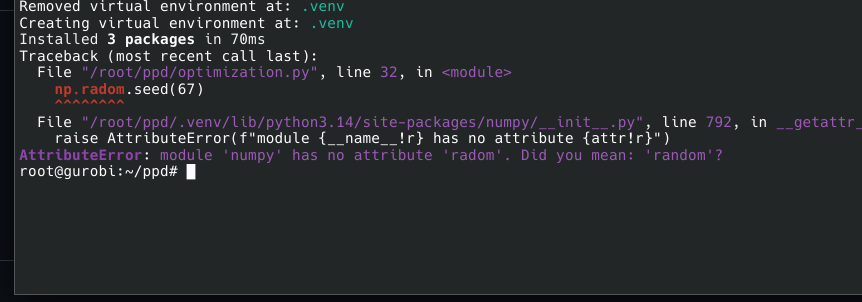
\includegraphics[width=0.5\linewidth]{radom.png}
\end{figure}


\end{document}


